\documentclass[article]{aaltoseries}
\usepackage[utf8]{inputenc}
\usepackage{algorithm}
\usepackage{algorithmic}


\begin{document}
 
%=========================================================

\title{Training deep neural network on mobile devices}

\author{Dongmin Wu
\\\textnormal{\texttt{dongmin.wu@aalto.fi}}} % Your Aalto e-mail address

\affiliation{\textbf{Tutor}: Jukka K. Nurminen} % First and last name of your tutor

\maketitle

%==========================================================

\begin{abstract}


  Since the Deep learning(DL) technology was published, this technology has been
  implemented in various fields and obtained exciting results. 
  However, this technology has considerable requirement of computational resources, especially
  in training phase. In addition, the large number of mobile devices makes the implementation
  of DL on mobile devices a promising topic. 
 According to the high dependency on computation resources,
 Mobile computing devices, such as mobile phone,
  wearable devices and tablet can rarely directly execute the training phase of DL. 
 Currently, there are already some solutions for implementing DL on mobile\cite{Ota:2017}
 but most of them are focusing on the predicting phase of DL. 
 Thus in this paper, we are focusing on the training phase of DL on mobile devices.
 This paper lists two major solutions currently used in implementing training phase of DL on mobile service;
 briefly introduces the features of both and talks about the scenario of the appliance. 

 ---------------------------------------------------------------
 
  %========move to intro
  The Deep learning technology can acquire 
  dependable abstractions from various data, which has benefited different applications, 
  including motion detection, natural language processing and image recognition. 
  Although some of the Deep learning technologies 
  has already reduced the complexity of neural networks to an acceptable size for web service, the 
 scale of the Deep learning technology is still large. 
 Discussing the learning phase of DL on mobile is necessary too, 
 it gives a neural network capability of self-evolution without strong help from backend services.



\vspace{3mm}
\noindent KEYWORDS: Deep learning, Mobile devices, Training phase, Knowledge Distillation, Federal Learning

\end{abstract}


%============================================================


\section{Introduction}


Deep learning has been widely used recently. As the main algorithm of Deep learning technology,
 the popularity of neural network algorithm 
 has considerably increased and become the state-of-art for solving different pattern recognition
problems.

The neural network is inspired by the neural system of the human brain. A neural network will 
try to model pattern of data by using a large number of intelligent nodes, which are named perceptrons. 
After gathering those computational units together, due to the high complexity of neural networks. 
This algorithm has the potential to fetch non-linear features from the training data 
and build a more precise pattern.

As the result, in the image, voice and complex pattern recognition fields, the performance of Deep learning
is generally better than other Machine Learning algorithms.  

However, some obvious issues appeared because of the large complexity of the Deep learning technology. 
Generally, Deep learning algorithms cost most during its training process. 
For example, a typical Convolutional Neural Network (AlexNet \cite{NIPS2012_4824}) 
spends approximately 2.6 minutes in a forward process for one image on a mobile device\cite{lane2015early}.
Due to the high computation requirement, Deep learning algorithms mainly run on the Graphics Processing Unit(GPU) or special processors, 

In addition, the energy consumption of Deep learning algorithms is also considerably large. %TODO: [example]

Deep learning also has widely usage scenarios on mobile devices, for example, mobile phones, 
wearable devices and vehicle electronics. Mobile devices have less computational resources than 
servers and large computers. On the other hand, mobile devices can hardly afford the energy consumption
of normal Deep learning algorithms. For solving those issues, some approaches appeared.

Ota et al.\cite{Ota:2017} comprehensively listed different Deep learning algorithms,
reviewed some software frameworks and hardware platforms for executing neural networks on mobile devices.
At last, they presented some applications running on mobile devices integrated with Deep learning technology. 
But they didn't mention the performance of training a Neural Network on mobile devices. 

%TODO: I should first list some solutions, and then explain that we will compare two of them
This paper will analyse the characteristics of Deep learning and neural network algorithms;
list the different methods of training NN on mobile devices and introduce those methods briefly. 
At last, this paper will give a conclusion by supposing some scenarios of the appliance.


In section \ref{sec:background}, we will introduce some background knowledge about neural network and mobile devices.
Section \ref{sec:related_works} shows some related works in the field of training Deep neural networks on mobile devices.
We present two main approaches currently used and introduces the detailed method in section \ref{sec:approaches}.
Finally, we make the conclusion and raise some possible future works.





%============================================================


\section{Background}
\label{sec:background}

In this section, the Deep learning and mobile devices will be introduced. This fundamental 
knowledge helps us to understand the context of this paper better.


%------------------------------------------------------------


\subsection{Deep Learning and neural network}

The neural network in Deep learning can be called Deep Neural Network(DNN), which is one of the most promising 
parts of current machine learning methods. 

\subsubsection{History of Deep Neural Network}

% 1. history  1page
In the mid-19th a paper was already introduced an Artificial Neural Network (ANN)\cite{Warren1943}, 
McCulloch et al. developed the first simple ANN which mimics the neural network system of the human brain. This ANN is not
able to learn models from data, but following research extended the capabilities of ANN and generated an unsupervised 
learning algorithm and supervised algorithm subsequently.

In the 1970s and 1980s, a back-propagation learning algorithm was found. Because of efficiency, the application of back-propagation
reached its peak in the mid-80s. LeCun applied this algorithm on the convolutional neural network 
for the first time in 1989, which had a significant impact on the Deep learning. After that, the Cresceptron Model was introduced, 
the using of max-pooling layers in the neural network architecture was widely used in the modern Deep learning technology.

After the year of 2010, Deep learning has another wave of popularity because there are more affordable Graphics Processing Units(GPU)
 with powerful parallel computation capacities. AlexNet\cite{NIPS2012_4824} earned the first prize of 
the 2012 ImageNet Large-Scale Visual Recognition Challenge (ILSVRC). 

From then on, the researching of DNN has considerably accelerated. Google, Facebook, Apple and Amazon has published
their own papers in this area. In 2015, Google introduced their GoogLeNet\cite{GoogLeNet}, whose Inception model composed the convolutional 
neural network in a new way such that no sequentially arranged layers are possible. In the same year, the ResNet\cite{ResNet} of Microsoft won 
the ILSVRC with the error rate of 3.6\%, which is smaller than the error rate of human beings.




\subsubsection{Characteristic of Deep Neural Network}
% 2. characteristic 1page

The Deep Neural Network has the higher hierarchy than ANNs, which means a large number of hidden layers\cite{MAL-006}. 
This difference makes DNN understand more complex models than ANN, which means the Deep learning or especially DNN
has better behavior on describing non-linear objects, including image, voice, text and bioinformatics.

Furthermore, compared to Machine learning technology, deep learning is more suitable for various tasks. The basic concept
of DNN is a multi-layer neural network, the algorithm will produce a pattern by itself only relies on a large data set.
On the contrary, previous machine learning algorithms specifically are designed for the specific tasks. 
With DNN technology, users can tackle different issues with one implementation of DNN. 

As the widely used of Big data technology, the old machine learning technologies such as Support Vector Machine (SVM) are
not such suitable for processing a large amount of data. On the other hand, because of the discovery of back-propagation
algorithm, the efficiency of DNNs is relatively higher than traditional Machine learning algorithms.

DNN is more flexible as well. Since the DNN consists of multiple neutrons, the number of neutrons can be adjusted
according to the requirement of different task. This characteristic allows DNN has a large potential of applying. So far, 
DNN has already impacted our life, services, e.g., Google translate, AlphaGo and Siri are the examples of successful applications.






%------------------------------------------------------------


\subsection{Current mobile devices} %2 pages

In this paper, the mobile devices are considered as a group of electronic devices with
computational units that has good mobility and provides the interactive features to human beings.
As the range of mobile is quite large, in this paper, we specifically discuss 3 representative 
mobile devices: Mobile phone, wearable devices and vehicle devices.




%history fo mobile devices
\subsubsection{History of mobile devices}

As the most common mobile devices in our daily life, the mobile phone is one of the most familiar 
electronics to normal people. For example, there are nearly 300,000 mobile phones have been 
sold during the second quarter of 2016 \cite{moblePhoneSale}. In 1973 the first handheld mobile phone
was showed by John F. Mitchiell and Martin Copper in America. Since then the mobile phone 
changed the modern life. In 2007, Apple Inc. published the first multi-touch smartphone,
 which made the mobile computation become true.
  Currently, almost all the mobile phones are in this form. 


Wearable devices, like Nike+, Google Glass and Apple watch are produced in the last decade. They present
a type of on-body electronics in addition to mobile phones. They mainly have specific features, some of them
are designed for monitoring body status while others have the limited interactive functionality.

The last category of mobile devices discussing in this paper is the vehicle devices. From the oldest vacuum tube
car radios to recent automatic driving systems, electronics in vehicles acted an important role while people
driving. Along with the development of mobile electronic technologies, the vehicle devices are becoming more convenient
and computational.



\subsubsection{Characteristic of mobile devices}

Because of the limited resources and specific usage, mobile devices, in general, do not have a high-performance 
universal computation core. Alternatively, they have some specifically designed computation units like DSP processor,
baseband processor and coprocessors.

In mobile phones, the power of processors considerably increased in past few years. But the limitation still existed, 
one of the main reason is the energy consumption. Mobile phones have limited size and need meet the requirement continually
using, that limitation makes the computation capability of mobile phones is relatively lower than desktop computers.

As for other wearable devices, they have more limited battery capacity and slower speed. In addition to that, 
they generally have more real-time requirement than mobile phones. Most of them are required to be able to monitoring
movement immediately.

Vehicle devices have the most computation resources comparing to the other two. Currently, some self-driving
cars are existed in the market, such as Waymo, most of them are driven by Deep learning technology. 
But safety requirement of vehicle devices is highest compared to another two devices.  



%------------------------------------------------------------





\section{Related works}
\label{sec:related_works}

To the best of our knowledge, except for hardware specific optimization like Apple's coreML\cite{AppleInc.},
 current solutions of squeezing the learning phase of Deep Learning on mobile devices 
are focusing on two directions: model compression and distributed learning.

\subsection{Model compression}

MobileNets\cite{MobileNets2017} is a compressed convolutional neural network discovered by Google. MobileNets developed 
from streamlined architecture, it performs nearly the same accuracy as the VGG16\cite{simonyan2014very} with 32 smaller
and 27 times less computational cost. MobileNets has a wide use case, e.g., object detection and face detection.

Han et al.\cite{Han2015} presented an approach of compressing the neural network in 2016. 
They deployed a 3 stage pipeline: pruning, trained quantization and Huffman coding, which is able to decrease
the size of the neural network from 35x to 49x. In addition, they compressed network increases the speed from 3 times to 4
and has 3x to 7x better energy efficiency.

\subsection{Distributed Learning}

Ananda et al.\cite{Suresh2016} show an optimization of the original naive distributed mean estimation algorithm, which uses 
stochastic binary rounding approach yields a mean squared error. They also improve the coding strategy to reduce the error.
Jeffery et al.\cite{NIPS2012_4687} achieve an algorithm which applies to any gradient-based 
machine learning algorithm named Downpour SGD.
Combining with Sandblaster, a framework, they are able to train a deep network 100x larger than before.





%------------------------------------------------------------


\section{Detail introduction of two approaches}
\label{sec:approaches}


% TODO: explain that there already some approaches, but this two of them are most representative. 



As last sections show, a large number of representative methods have been discovered in the model compression and distributed learning. 
In this section, two methods will be discussed:
Reducing the size of a mentee Neural Network and Increasing the capability through distributed computation.


\subsection{Reducing the size of a mentee Neural Network}

In 2014, \emph{Knowledge Distillation}, an approach to reducing the size of Neural Network, 
showed an idea of teaching a new simpler Neural Network with a well-trained complex Neural Network.
Within that way, a representative Neural Network was formed and the size is small enough for mobile training.

Figure \ref{fig:mentor_pic}\cite{Distillation:2015} shows the schematic of this mentee-mentor architecture. 

\begin{figure}[t!]
  \begin{center}
    % Note how the file extension has been removed from the filename below
    % so that the LaTeX command can automatically pick any supported file format
    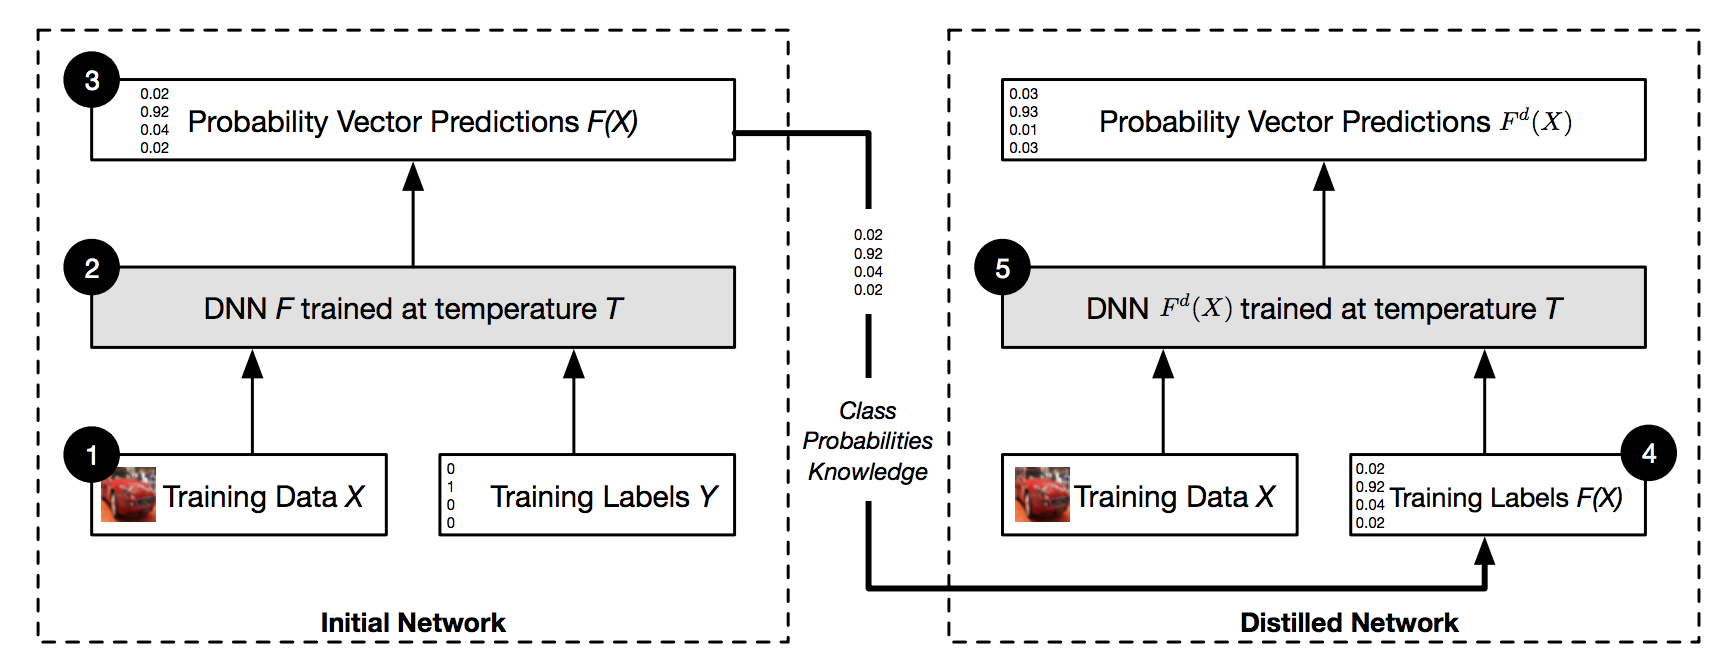
\includegraphics[width=1\textwidth]{figures/mentor_mentee}
    \caption{The mentee network uses the outputs of mentor network as its input labels}
    \label{fig:mentor_pic}
  \end{center}
\end{figure}

As the figure shown, the mentee network has much fewer layers of Neural Network. 
Hinton et al.[reference], presented the Knowledge Distillation that makes neural network smaller by learning the 
output of the softmax layer\cite{SoftMax}. 

This idea was originally introduced by \cite{Caruana2006}, the paper showed 
the output of the softmax layer have much more information than a simple classifier. 
The softmax function is also able to show the correlations between
target labels. For example, in a computer image recognition neural network for classifying cat, dog and boat.
If the input of that network is a picture of a cat, the correlation of the output
between cat and dog is higher than cat versus boat because the appearance of a cat is more similar to a dog than a boat.
Hinton called those hidden information in the softmax output as \emph{Dark Knowledge}, 
as the knowledge is unused and ignored by normal neural network classifier.

Base on the phenomenon above, a smaller mentee neural network can get a more accurate result with the regularization from
the Dark knowledge. 
The approach of \emph{Knowledge Distillation} mainly has two steps: target soften and distillation.

\subsubsection{Target soften}

Normally, for a data set \(X\), we can derive features \(\textbf x \) and correspond target labels \(\textbf y\).
In addition, we can get the predicted output vector \(\textbf y_{mentor}\) from the mentor network.
The parameters in the mentor network are \(\Theta_{mentor}\), 
the derivation of \(\textbf y_{mentor}\) can be represented as below:

%TODO: not sure the equation is correct
%TODO: add softmax function
\[
  \textbf y_{mentor} = softmax(\Theta_{mentor} \textbf{x})
\]

In the practical, the target labels are collected in a format named one-hot, a term comes from the digital
design field\cite{DigitalDesign}. For example, if \(X\) has three target labels: \emph{cat, dog} and \emph{car},
The target labels \(\textbf{y}\) will be presented in following format:

\[
  cat:\ y = \{1,0,0\};\ 
  dog:\ y = \{0,1,0\};\ 
  car:\ y = \{0,0,1\};\ 
\]

The one-hot form above was defined as the \emph{hard target}, as they only reveal the classification result of input data.

However, a prediction of a well-trained mentor network \(\textbf y_{mentor}\) will show as a value between 
\(0\) and \(1\), because of the softmax layer of the neural network. 

\begin{equation} \label{eq:cat_example}
  cat:\ y_{mentor} = \{0.9,0.2,2 \times 10^{-6}\}
\end{equation}

Above is an example output with an input of cat image, 
the first item is obviously highest and the second item is relatively higher than the third.


In the target soften step, 
the output from complex mentor network \(\textbf y_{mentor}\) will soften in order to get the correlation between categories
by replacing the softmax function as below.

\begin{equation} \label{eq:new_soft_max}
  f(z_{(i)}) = \frac{exp(z^{(i)}/T)}{\sum_{j=0}^{N}exp(z^{(j)}/T)}\ for\ i=0,1,...,N
\end{equation}

There, \(T\) represents the "\emph{temperature}" of the soften procedure, a larger \(T\) leads to a more average result. 
If \(T =1\), the equation \ref{eq:cat_example} is the same with normal softmax function. 


\subsubsection{Distillation}

The aim of distillation is to transfer the knowledge from the larger mentor neural network to the mentee. 
The mentee will use the output of the mentor with high temperature as the target labels.
Equally, the softmax layer of the mentee neural network has the same temperature with its mentor.

As the result, the cross-entropy between the mentee and mentor presents as:

\begin{equation} \label{eq:cost_function}
  C(y_{mentee}, y_{mentor}) = - \sum y_{mentor}log(y_{mentee})
\end{equation}

Insert equation \ref{eq:new_soft_max} into equation \ref{eq:cost_function}, we can derivate below:

\begin{equation} \label{eq:cost_function1}
  C(y_{mentee}, y_{mentor}) = - \sum_i f(v_i)log(f(z_i))
\end{equation}

There, \(v_i,\ z_i\) presents the input of mentor and mentee's softmax layer respectively.

Thus, the gradient of equation \ref{eq:cost_function1} is:

\begin{equation} \label{eq:gradient_cost}
  \frac{\nabla C}{\nabla z_i} = \frac{1}{T}(f(v_i) - f(z_i))
\end{equation}

Expand equation \ref{eq:gradient_cost}, while \(T\) is large enough, the equation transform into below:

\begin{equation} \label{eq:gradient_cost1}
  \frac{\nabla C}{\nabla z_i} \approx \frac{1}{T}( \frac{1+z_i/T}{N+\sum_j z_i/T} - \frac{1+v_i/T}{N+\sum_j v_i/T} ) = \frac{1}{T} (\frac{z_i - v_i}{N})
\end{equation}

Within the cost function \ref{eq:cost_function1} and the gradient equation \ref{eq:gradient_cost1}, 
the mentee neural network can learn the knowledge from its mentor.

The Dark Knowledge introduced a good approach to mobile training. 
A large and well-trained Neural Network, which has a general knowledge of a scenario, can be computed and stored in the powerful server cloud.
At the meantime, a small mentee network regularized by the mentor network can be stored and adjusted on the mobile devices.
For a specific use case, the mentee network is able to learn from that and adjust the predicted result. 



% Maybe I can move this part to another section
The advantage of this method is obvious, 
the size of mentee network is much smaller than the mentor network but has similar performance
with the complex mentor network. 
Although this compression is efficiency, the mentee network can still too large for some mobile
devices such as wearable devices.


\subsection{Federal learning among multiple mobile devices}

Google also published \emph{Federal Learning} for solving the issue of training models on mobile devices.
Their approach tries to train a neural network in multiple mobile phones, each phone only trains a few iterations
and all the tuned parameters of the neural network will be integrated by the server. 
This approach makes the training on the mobile devices possible.

In 2010, Zinkevich et al.\cite{Zinkevich2010} discovered a method of utilizing multiple machines to parallelize the gradient descent.
In their approach, the whole system comprises a server and several clients. 
The clients will only train one iteration with one batch of data by using Stochastic Gradient Descent(SGD) algorithm, 
then the server will combine all the calculated weight parameters and computes the average value of parameters.
This algorithm is called one-shot averaging because clients will only train one iteration with one batch.

One-shot averaging exists some issues, one of them is that in some case the performance will be worse than training
the model on one computer\cite{Shamir2013}. In addition, one-shot averaging costs a multitude of communication resources
due to the averaging step need to be performed every time after calculating the gradient.


To overcome those issue, the \emph{Federal Learning} mainly uses two methods: \emph{Federal Averaging} 
and shared initial weight.

\emph{Federal Averaging} is an optimization of one-shot averaging, the algorithm controls the distributed learning process by
three parameters: $C$ presents the fraction of clients that calculate gradient descent on each round; $B$ is the minibatch size
while client performs the computation; $E$ indicates the amount of training executed on each round.
On each round of \emph{Federal Averaging}, a number of $C$ clients will be randomly selected, performing $E$ times gradient
descent, and finally return the updated weight parameters back to the server node. As the clients will update the 
weight parameters several $E$ times before return the result to the server node, this method decreases the communication cost.
Figure \ref{alg:FederalAveragingAlgorithm} presents a pseudo-code of \emph{Federal Averaging}, all initial weight was shared already.


\begin{figure}[t!]
  \begin{center}
    % Note how the file extension has been removed from the filename below
    % so that the LaTeX command can automatically pick any supported file format
    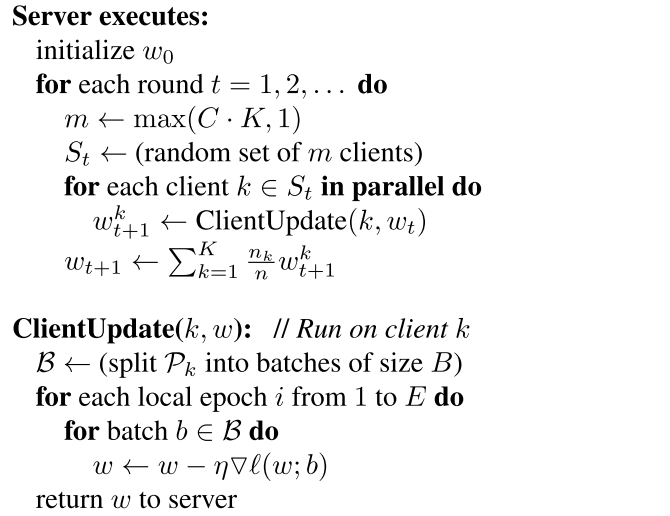
\includegraphics[width=0.6\textwidth]{figures/Algorithm}
    \caption{Federal Averaging. The $K$ clients are indexed by $k$; $B$ is the local minibatch size, 
            $E$ is the number of local epochs, and $η$ is the learning rate.}
    \label{alg:FederalAveragingAlgorithm}
  \end{center}
\end{figure}


The shared initial weight is an empirical method found by authors. They found that starting the models with the same random
value will lead to a good optimization even though the models were trained independently with two different subsets of the data.
Figure \ref{fig:share_weight} shows the result of training the same MNIST dataset \cite{lecun2010mnist} without and within the 
shared initial weight methods. 
Within this method, averaging the models have a considerably small loss over the training set.

\begin{figure}[t!]
  \begin{center}
    % Note how the file extension has been removed from the filename below
    % so that the LaTeX command can automatically pick any supported file format
    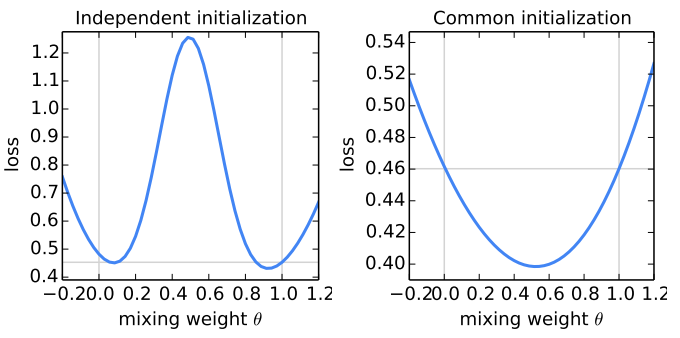
\includegraphics[width=0.7\textwidth]{figures/share_weight}
    \caption{The left independently initialize the weight; in the right case, the models were initialized by the same seed.}
    \label{fig:share_weight}
  \end{center}
\end{figure}

With the \emph{Federal Learning}, we are able to reduce the communication cost and distribute the computation resources into multiple,
without a significant loss.
This technique makes the training on the mobile device available, Google already tested the \emph{Federal Learning} with Google's keyboard
on Android devices\cite{BrendanMcMahanandDanielRamage2017}.

%------------------------------------------------------------




%============================================================


\section{Conclusion and Future Work}
\label{sec:conclusion}

This paper firstly introduces what is Deep learning and neural network; shows the current situation of this technology;
lists the background and challenges on training Deep Neural Network. Additionally, two state-of-art approaches were 
presented as possible solutions of implementing training neural network on mobile devices. \emph{Knowledge Distillation} 
is focusing on generating a smaller equal neural network which can run on the limited computational devices; 
\emph{Federal Learning} raises a solution that distributes the computational capability, makes the training process
extendable. 

`'
The two approaches solving the challenges in a different way, which means they have the possibility to integrate together. 
The combination of those will be an interesting goal for the future work. 

%TODO: add disadvantage of dark knowledge/knowledge Distillation
%TODO disadvantage of knowledge distillation
%   1. the performance is bad on small set of categories
%   2. not efficient on GAN neural network


%============================================================


\bibliographystyle{plain}
\bibliography{cs-seminar}

\end{document}
